\section{React}
\setauthor{Michael Ruep}
The frontend of SeatGen is built using the React framework. This choice was primarily motivated by the existing expertise within Solvistas, ensuring that the company’s developers could easily maintain and adjust the project to their needs. Additionally, React provides an ideal balance between flexibility, performance, and a vibrant ecosystem, which are factors that proved crucial when building an interactive seating plan editor for stadiums. Also, our team was already experienced with component-based single page application frontend frameworks.

\subsection{Framework Background}
React is an open-source JavaScript library developed and maintained by Meta (formerly known as Facebook) and a community of individual developers and companies. Originally introduced in 2013 to power Facebook’s dynamic news feed, React has since become renowned for creating data-driven web interfaces~\cite{ReactDocs, SPAComp}. Rather than manually manipulating the Document Object Model (DOM), developers can simply declare how the interface should appear based on the underlying data. This declarative approach allows React to handle updates internally, ensuring smoother user interactions, which are especially beneficial for large or frequently changing data sets~\cite{ReactVirtualDOM, SPAComp}.

\subsection{Virtual DOM}
\setauthor{Michael Ruep}
React’s Virtual DOM architecture is particularly advantageous for applications requiring frequent updates and complex UI interactions. In SeatGen, each seat on the map can be added, moved, or deleted in real time, causing rapid changes that must be reflected in the user interface without compromising speed. By selectively re-rendering only components that have actually changed, the Virtual DOM mechanism helps maintain excellent performance even under heavy load~\cite{ReactVirtualDOM}. This aligns with the findings in~\cite{SPAComp}, where React demonstrates superior rendering speed and user satisfaction in Single Page Applications (SPAs) requiring dynamic content updates.

\subsection{Component-based Architecture}
\setauthor{Michael Ruep}
React’s component-based architecture keeps each feature modular to make the project easier to maintain as it grows. Instead of bundling all functionality into a single monolithic view, UI features are developed as self-contained components. In our case for example:
\begin{compactitem}
    \item Seat Map Component
    \item Toolbar Component
    \item Detail Component
\end{compactitem}
Each of those elements has its own component, allowing developers to modify or expand individual features without affecting unrelated parts of the application. This approach simplifies debugging, since issues can often be traced to a specific component rather than across the entire codebase. It is also suitable for collaborative development by letting team members work on separate components in parallel, which significantly accelerated our development process. Overall, React’s modular design reduces complexity which assists a more organized and maintainable codebase.
~\cite{ReactCBA01, ReactCBA02, ReactCBA03}

\subsection{Integration of Libraries}
\setauthor{Michael Ruep}
One of SeatGen’s central requirements is to enable direct manipulation for seat layouts. React’s flexible architecture allows us to easily incorporate third-party libraries. For example, we integrated Leaflet to render the stadium map using its efficient, canvas-based engine. React uses its Context API to manage global state and user interactions, while Leaflet is responsible for the map rendering. This separation ensures that intensive mapping operations do not interfere with overall UI responsiveness. We used Reacts Context to manage global state effectively, rather than relying on more complex solutions. This approach meets the specific requirements of seat manipulation, multi-layered zoom levels, and user interactions.

\subsection{Developer Familiarity and Team Expertise}
\setauthor{Michael Ruep}
Since React was already in use at Solvistas, its adoption ensured that the company’s developers could seamlessly work with and extend the project. Additionally, our team had prior experience with component-based frontend frameworks, making it easy to understand React’s structure, including concepts such as routing, state management, data binding, and components. This familiarity allowed us to quickly understand and use React, and we immediately had our first running prototype.

\subsubsection{Comparison to Other Frameworks}
\setauthor{Michael Ruep}
Compared to alternative frameworks such as Angular or Vue studies have shown that React and Vue generally demonstrate superior rendering performance and faster load times in dynamic applications~\cite{SPAComp}. Additionally, React is preferred by developers for SPAs with frequent UI updates, with a reported 34\% higher satisfaction rate compared to other frameworks~\cite{SPAComp}. 

\subsection{Summary}
\setauthor{Michael Ruep}
React’s widespread adoption, strong ecosystem, and proven efficiency in building dynamic web applications make it a reliable choice for modern frontend development. Its Virtual DOM ensures optimized rendering performance, while its component-based architecture keeps the application modular and maintainable. Additionally, React Context provides a lightweight yet effective solution for managing global state. This allows seamless integration with external libraries such as Leaflet for real-time seat rendering~\cite{ReactVirtualDOM, ReactCBA01}. 

With React already in use within the company, adopting it ensured maintainability and smooth collaboration. Its performance advantages in Single Page Applications (SPAs), along with high developer satisfaction rates~\cite{SPAComp}, further validated its suitability for our interactive seating plan editor.

\section{Spring Boot and Kotlin}
\setauthor{Michael Stenz}
For the backend logic, Spring Boot was chosen as it is a core technology in Solvistas' tech stack. This decision ensures that the project remains maintainable by Solvistas developers in the long run. The backend has several key responsibilities, including:\begin{compactitem}
    \item Handling the storage of the seatplan metadata
    \item Converting SVGs into image tiles
    \item Uploading the converted tiles to an S3 bucket
    \item Serving all of this data to the frontend via REST
\end{compactitem}

For image processing tasks such as resizing and slicing SVGs and PNGs, Python was initially considered due to its well-documented and easy-to-use image manipulation libraries like CairoSVG and OpenCV. However, the decision was ultimately made to keep the processing within the Java/Kotlin ecosystem, using libraries like Batik and ImageIO. While Java/Kotlin image processing is not as straightforward as Python due to less extensive documentation and fewer community resources, this choice allowed for a consistent backend technology stack. One challenge with Java-based image processing is memory management—heap size and garbage collection must always be considered, especially when processing large images. For file uploads, Amazon S3 provides excellent support for Java and Kotlin through the AWS SDK, accompanied by extensive documentation and examples. This integration made it easy to incorporate S3 into the backend for efficiently storing and retrieving image tiles.

\subsection{Kotlin}
As for the language, Kotlin was used in Spring Boot, even though it is not commonly employed in many of Solvistas' projects. However, Kotlin was deemed the better option because it is a modern language that is fully interoperable with Java and offers many features that facilitate writing clean and concise code, thereby reducing errors and improving readability and maintainability. It eliminates much of the boilerplate code required in Java and provides a rich standard library with numerous built-in utility functions, significantly reducing development time. While Kotlin does not offer essential functionalities that Java cannot provide, it is more modern and has a more concise syntax.

Additionally, Kotlin introduces powerful features such as null safety, which helps create more robust applications with fewer runtime errors. Furthermore, Kotlin provides strong support for functional programming, including higher-order functions, lambda expressions, and extension functions, making it easier to write expressive and reusable code. Another key advantage is Kotlin’s coroutines, which enable highly efficient asynchronous programming without the complexity of Java’s traditional thread management. This makes Kotlin particularly well-suited for handling concurrent tasks, such as processing multiple image transformations simultaneously, significantly reducing processing time.

Kotlin’s seamless integration with Spring Boot also allows for idiomatic DSLs (Domain-Specific Languages), which can simplify configuration and reduce verbosity in code. The language’s structured concurrency and intuitive syntax contribute to cleaner, more maintainable backend services, ensuring long-term scalability. Finally, Kotlin’s growing adoption within the Spring ecosystem, along with first-class support from JetBrains and the Spring team, makes it a viable choice for modern backend development. Its developer-friendly nature, combined with reduced verbosity and enhanced safety features, positions it as a forward-thinking investment despite its lower adoption within Solvistas' existing projects.

In the end, Spring Boot with Kotlin was chosen due to the team's expertise with the language and the fact that all other components of the Ticketing software were already written in Spring Boot.

\subsection{API Documentation with Swagger}
SeatGen also utilizes SwaggerUi and SwaggerUi codegen to generate REST API documentation and client code for the frontend. This allows for easy integration of the backend with the frontend and ensures that the frontend developers always have the most up-to-date API documentation. This is done via the OpenApi gradlew plugin, which generates the SwaggerUi documentation and client code for all the API endpoints and required models. The generated docs can be fetched by the frontend developers with a script within the \texttt{package.json} file, under the name \texttt{fetch-openapi-docs}. This script fetches the api-docs.yaml file from the backend and saves it in the frontend project. When starting or building the frontend, the \texttt{swagger-typescript-api} plugin generates the client code from this file. The frontend developer now can use the generated client code to interact with the backend API through the generated functions and models without having to manually maintain the API client code.


\section{Database}
\setauthor{Michael Stenz}
PostgreSQL was chosen as the database for several key reasons. A relational database is required since the data follows a structured design that is best represented through classical relational models. The structure of the database is visualized in the class diagram \ref{fig:db_model}. Additionally, utilizing a relational database simplifies the process of exporting generated data into the Ticketing database, which also adheres to a relational structure.

\begin{figure}
    \centering
    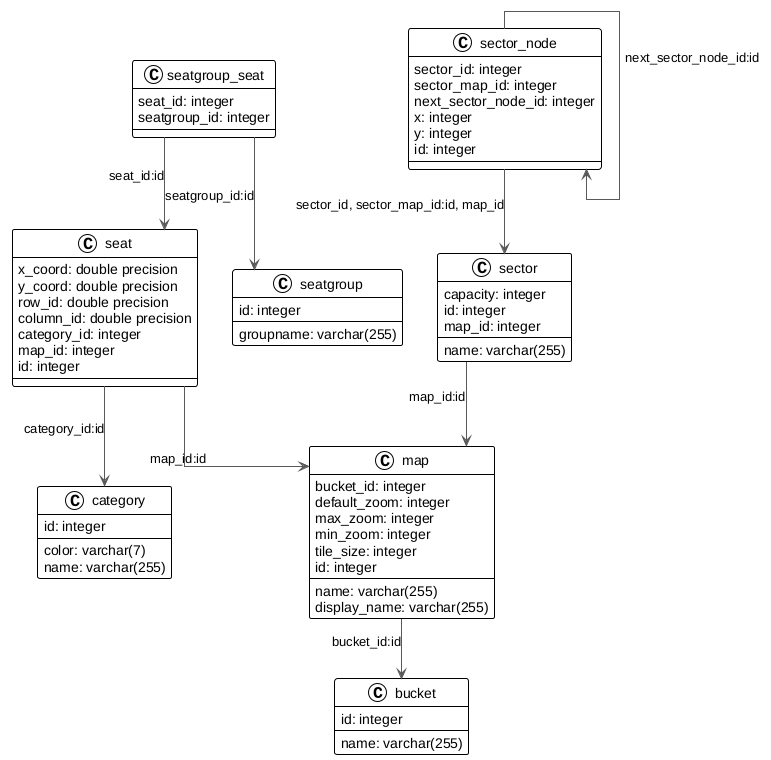
\includegraphics[scale=0.5]{pics/db_model.png}
    \caption{Database Model}
    \label{fig:db_model}
\end{figure}

The system is designed to be compatible with multiple relational databases, not just PostgreSQL, as the Java Persistence API (JPA) is utilized as the Object-Relational Mapping (ORM) framework. To maintain database flexibility, PostgreSQL-specific commands were deliberately avoided. While leveraging PL/pgSQL for business logic could have provided benefits such as enhanced security, improved performance, and greater data consistency, database interchangeability was prioritized.

For database connectivity in the Spring Boot application, the Spring Data JPA library was utilized. This library streamlines the process of connecting to a database and executing queries while implementing the repository pattern. Through this pattern, custom queries are defined in an interface, which Spring Boot automatically implements at runtime. This approach simplifies query management, making it easier to maintain and use repository methods directly within the codebase.

To manage database migrations efficiently, the Flyway library is used. Flyway enables the to define database changes through SQL scripts that execute automatically when the application starts. This ensures that the database schema remains consistent with the latest changes, simplifying deployment and mitigating potential conflicts across different environments. Managing migrations this way also helps prevent issues arising from different database versions among team members. Additionally, since Flyway migrations consist of entire SQL scripts, both Data Definition Language (DDL) and Data Manipulation Language (DML) commands can be executed. This capability is particularly beneficial for tasks such as migrating data between tables, altering column data types, and implementing other business logic-related transformations.

When selecting a migration tool, both Liquibase and Flyway were evaluated. While both are open-source and provide seamless integration with Spring Boot and other Java frameworks, the decision was ultimately made to opt for Flyway due to its simplicity and specific use case. Since the team is small with infrequent parallel database changes, Flyway’s linear migration approach suits the workflow without introducing complications. Although this approach might present challenges in larger teams with concurrent database modifications, it remains a practical choice for current needs.

Flyway also offers a cleaner versioning system by requiring migration filenames to follow a structured naming convention: \texttt{VX.X.X\_\_migration\_name.sql} (where X.X.X is the version of the migration). In contrast, Liquibase utilizes changelog files, which provide additional features but introduce unnecessary complexity for the use case. These changelog files can be written in SQL, XML, YAML, or JSON, but they require extensive Liquibase-specific formatting. The following example illustrates a Liquibase-formatted SQL changelog file \ref{lst:liquibase:example}. Flyway's approach, which relies on plain SQL migration files, enhances readability and maintainability.

\begin{lstlisting}[language=Sql,caption=Liquibase example changelog,label=lst:liquibase:example]
    --liquibase formatted sql
    
    --changeset nvoxland:1
    create table test1 (  
        id int primary key,
        name varchar(255)  
    );  
    --rollback drop table test1; 
    
    --changeset nvoxland:2 
    insert into test1 (id, name) values (1, 'name 1');
    insert into test1 (id,  name) values (2, 'name 2');  
    
    --changeset nvoxland:3 dbms:oracle
    create sequence seq_test;
\end{lstlisting}
    
To ensure database consistency, Flyway generates a flyway\_schema\_history table that tracks all executed migrations. This table stores metadata for each migration, including the version, description, execution timestamp, and a checksum. The checksum prevents modifications to previously applied migrations, ensuring consistency but potentially causing unexpected errors during local development. In such cases, manual intervention in the flyway\_schema\_history table may be required, but except for these rare cases the flyway\_schema\_history table should not be manipulated manually.

By maintaining this history, Flyway can determine which migrations have been applied and which are still pending. Each migration also has a state, which can be pending, applied, failed, undone, and more—detailed in the Flyway documentation. These states allow system administrators to quickly identify and resolve migration and deployment issues.

When considering how to store image data, PostgreSQL’s built-in options, including BLOBs (Binary Large Objects) and TOAST (The Oversized-Attribute Storage Technique), were evaluated. While these mechanisms allow PostgreSQL to handle large binary files, the decision was ultimately made against using them due to performance concerns, maintenance overhead, scalability limitations, and company reasons.
Even though, TOAST is very performant and automatically compresses and stores large column values outside the main table structure, making it a more attractive option than traditional BLOBs, accessing and manipulating the stored images via SQL queries can become a bottleneck. ORMs like Hibernate tend to retrieve large column values by default unless explicitly configured otherwise, potentially leading to performance degradation when dealing with frequent queries. This means extra effort would be required to optimize database queries to avoid unnecessary data retrieval, increasing development complexity.


\section{AWS - S3}
\setauthor{Michael Stenz}
For image processing tasks such as resizing and slicing SVGs and PNGs, Python was initially considered due to its well-documented and easy-to-use image manipulation libraries like CairoSVG and OpenCV. However, the decision was ultimately made to keep the processing within the Java/Kotlin ecosystem, utilizing libraries such as Batik and ImageIO. While image processing in Java/Kotlin is not as straightforward as in Python due to less extensive documentation and fewer community resources, maintaining consistency within the backend technology stack was prioritized. One challenge associated with Java-based image processing is memory management—heap size and garbage collection must always be considered, especially when processing large images. For file uploads, Amazon S3 provides excellent support for Java and Kotlin through the AWS SDK, with extensive documentation and examples. This facilitated seamless integration of S3 into the backend for efficient storage and retrieval of image tiles.

In the Ticketing project, all image tiles are stored in an AWS S3 bucket. S3 was required due to its robust performance, reliability, and seamless integration with the AWS ecosystem, which is already in use at Solvistas. By utilizing the Amazon S3 SDK, the file upload process is automated, reducing manual effort and minimizing the risk of errors.

Using S3 also improves frontend performance by ensuring that image retrieval does not depend on the backend server’s speed. Instead of acting as a middleware for serving images, the backend delegates this task directly to S3, reducing its workload and enhancing response times.

AWS S3 was the only option considered, as it is the cloud platform used by Solvistas, and the infrastructure costs are funded by the company.

\section{Leaflet}
\setauthor{Michael Ruep}
Leaflet is an open-source JavaScript library designed for interactive maps. Developed by Vladimir Agafonkin and maintained by a large community, it is widely used for its lightweight nature and ease of integration with modern web applications~\cite{Leaflet}. Unlike heavyweight mapping solutions such as Google Maps or OpenLayers, Leaflet is specifically optimized for rendering custom vector layers and handling dynamic user interactions efficiently. These characteristics make it an ideal choice for SeatGen’s stadium seat visualization, where real-time updates and performance optimization are critical.

\subsection{Why We Chose Leaflet}
\setauthor{Michael Ruep}
For SeatGen, choosing the right mapping library was crucial to ensuring smooth and interactive seat visualization. Leaflet was selected due to its lightweight architecture, extensibility, and strong performance when rendering custom vector layers. Unlike Google Maps or OpenLayers, which offer extensive GIS (geographic information system focused) functionalities but often introduce unnecessary overhead, Leaflet is designed for fast, customizable, and lightweight mapping solutions~\cite{Leaflet}. 

A key advantage of Leaflet is its low dependency footprint. Unlike other mapping solutions that rely on external APIs or heavy SDKs, Leaflet provides a standalone JavaScript library that integrates seamlessly with React. This lightweight approach gives us great map performance, even when handling large stadiums with thousands of seats. In contrast, frameworks like Google Maps API enforce rate limits and external API calls, which can introduce latency and unnecessary costs.

Leaflet’s customizability also played a significant role in our decision. SeatGen requires custom zoom levels, and real-time updates, all of which are efficiently handled using Leaflet’s open architecture. Unlike proprietary mapping tools, Leaflet allows full control over rendering logic, making it easier to optimize performance and adjust the visualization to match stadium layouts precisely~\cite{Leaflet}. Furthermore, we adapted existing Leaflet functions for tasks such as seat selection and the grid tool. This significantly accelerated the development process

By selecting Leaflet, we ensured that SeatGen could efficiently handle multi-layered rendering, interactive zoom, custom maps, and seamless seat selection, all while maintaining a lightweight and scalable frontend architecture.

\subsection{Key Features Used in SeatGen}
\setauthor{Michael Ruep}

Leaflet provides several core functionalities that are essential for our interactive seating plan editor. The following features were particularly valuable in implementing a performant and user-friendly seat visualization system:

\begin{itemize}
    \item \textbf{Dynamic Seat Rendering:} Leaflet allows us to render thousands of seat markers efficiently without significantly impacting performance. Since stadiums can contain a large number of seats, we optimized rendering using Leaflet layers to manage visibility at different zoom levels.
    \item \textbf{Custom Zoom Levels and Scaling:} Leaflet enables us to define custom zoom levels. This ensures that users can zoom in for precise seat selection or zoom out to get a full view of the stadium’s structure.
    \item \textbf{Interactive Seat Selection:} By leveraging Leaflet’s built-in event handling system, we allow users to click and modify seats in real time. This is crucial as it enables us to intuitively adjust seating arrangements.
    \item \textbf{Grid-Based Seat Placement:} Leaflet’s selection, polygon, and coordinate functions were used to implement functions like the grid tool and selection tool, allowing for structured seat placement. This feature speeds up the process of generating rows and sections by automatically aligning seats according to predefined parameters.
    \item \textbf{Real-Time State Management with React Context:} Since Leaflet does not natively integrate with React’s state management, we used React Context to synchronize seat selections, updates, and modifications across the application. This ensures that any seat change is reflected immediately in both the UI and the underlying data model.
\end{itemize}

These features collectively make Leaflet a powerful tool for handling the seat visualization requirements. By leveraging Leaflet’s efficient rendering engine and customization capabilities, we created a seamless user experience that allows for real-time adjustments and intuitive stadium navigation.

\subsection{Integration with React}
\setauthor{Michael Ruep}
Integrating Leaflet with React was straightforward thanks to React Leaflet, a library that provides React components for Leaflet~\cite{ReactLeafletDocs}. This greatly simplified the integration process, as we could manage Leaflet elements within React components without direct manipulation of the DOM.

One challenge we faced was handling state management and data binding between Leaflet and React. Since Leaflet operates independently from React’s Virtual DOM~\cite{ReactLeafletDocs}, synchronizing real-time seat selections, modifications, grid placements and so on required a structured approach.

Beyond standard Leaflet functionality, we also extended and customized existing Leaflet features to meet our specific needs. Tools such as the seat selection tool and grid tool, leveraged Leaflet’s built-in functions but were adapted and modified to SeatGen’s requirements. By understanding and modifying Leaflet’s core functions, we were able to create a tailored solution that aligned with our requirements for real-time seat arrangement and stadium visualization.

\subsection{Summary}
\setauthor{Michael Ruep}

Leaflet’s lightweight architecture, flexibility, and strong customization capabilities made it the ideal choice for an interactive seating plan editor. Unlike heavier GIS-focused alternatives, Leaflet provided a high-performance mapping solution tailored for real-time seat rendering and selection. 

Its custom zoom levels allowed us to create an intuitive and responsive seating visualization tool. Additionally, React Leaflet streamlined the integration process, enabling us to build faster within React~\cite{ReactLeafletDocs}.

By leveraging Leaflet’s existing functionality while extending its core features to suit stadium seat planning, we ensured a clean, efficient tool suite and smooth real-time interaction. This makes Leaflet an essential part of our frontend architecture.